\chapter{基于变分推断的高效句法分析方法}
\label{cha:vi}

本章节在提出了章节~\ref{cha:dep-crf}和~\ref{cha:con-crf}提出的高阶句法解析器的基础上,尝试利用基于平均场变分推断来近似得到树的后验概率,并与精确推断的CRF相比较.
我们在依存句法和成分句法的中英文常见的5个基准数据集上做了实验,并对比了加入BERT之后的效果.
结果表明,我们采用的变分推断近似方法不仅从准确率上可以与章节~\ref{cha:dep-crf}和~\ref{cha:con-crf}里提出的二阶基于图的解析器相匹敌,并且训练和测试的速度要远远快于二阶CRF解析器.

\section{引言}\label{sec:vi-intro}
近年来句法分析领域有了长足的进步.
研究者针对句法分析任务提出了一系列的方法\citep{dozat-etal-2017-biaffine,gomez-rodriguez-vilares-2018-constituent,ji-etal-2019-graph,zhang-etal-2020-fast,wei-etal-2020-span},将英语基准数据集宾州树库(Penn Treebank, PTB)的准确率刷新到了很高的水平.
本章中我们主要关注于基于图的句法分析方法.

基于图的方法选择将一棵句法树分解为多个部分,然后分别打分,组成树的分值,并训练模型使得能够找到分值最大的句法树.
其中最简单的一阶方法让树中的每个变量都互相独立.
在深度学习时代之前,一阶方法通常需要结合结构化学习\citep{mcdonald-etal-2005-online,koo-etal-2007-structured,taskar-etal-2004-max}.
得益于深度神经网络的强大上下文建模能力,近期的一些工作通常基于更简单的训练方法,其中\citet{dozat-etal-2017-biaffine}(Biaffine Parser)提出一个简单的基于头选择目标的解析器,训练时最大化每条弧的头的概率.
\citet{gaddy-etal-2018-whats}则提出一个基于二分类目标的成分句法分析方法,训练模型判断每个可能位置是否组成组块.
由于其高效率,并且取得了不逊色于结构化学习方法的结果\citep{zhang-etal-2019-empirical,falenska-kuhn-2019-non},这些方法是目前最为流行的句法分析方法.

与此对应的,研究者通常也尝试更多结构化约束引入神经网络模型中.
一方面利用TreeCRF、Max Margin\citep{ma-hovy-2017-neural,falenska-kuhn-2019-non,stern-etal-2017-minimal}等结构化学习算法来全局最大化句法树的概率.
另一方面,则是尝试利用高阶特征,建模兄弟、祖父等子树结构\citep{mcdonald-pereira-2006-online,koo-collins-2010-efficient}.
我们在章节~\ref{cha:dep-crf}和章节~\ref{cha:con-crf}的工作证明,在神经网络模型中,引入结构化学习给句法分析任务会给带来了一定的提升.
在依存句法分析中我们还进一步尝试了二阶兄弟特征的高阶句法分析,是依存分析的结果超越了一系列前人的工作,达到了最佳水平.

尽管在神经网络上被证明有效,高阶结构化学习方法的一些固有缺陷限制了其应用.
由于需要精确推断得到树概率,这需要$O(n^3)$的时间复杂度,因此大大慢于一阶方法.
此外,如果进一步考虑其他高阶特征,例如共同父亲等等,这可能会导致动态规划结构难以设计,或者算法复杂度难以忍受.

考虑到这种限制,因此,在本章中我们参考前人的一些工作\citep{smith-eisner-2008-dependency,wang-etal-2019-second,wang-tu-2020-second},在利用高阶特征的同时,尝试用平均场变分推断(Mean Field Variational Inference, \textsc{Mfvi})方法来近似获得后验概率.
在本章中,我们在依存句法分析和成分句法分析这两个句法分析任务上尝试了应用基于变分推断的近似学习算法.
针对依存解析和成分解析两种任务的特性,我们分别在依存句法的变分推断中参考\cite{wang-tu-2020-second}引入了头选择的结构约束,而在成分句法中则采用了二分类的学习目标.
我们发现近似算法在获取了和精确推断接近的准确率的同时,解析速度能够大大提高.

% 近似方法\citep{smith-eisner-2008-dependency,gormley-etal-2015-approximation},并使用$AD^3$\citep{martins-etal-2011-dual,martins-etal-2013-turning}来进行解码.
总体而言,我们在本章节的工作如下:
\begin{itemize}
  \item 我们提出在句法分析任务上应用引入二阶特征的变分推断方法近似得到后验概率来进行结构化学习,并和前述章节的精确推断方法做了比较.
  \item 针对依存句法分析和成分句法分析任务的特性,我们分别探索了基于头选择的变分推断方法和基于二分类的变分推断方法用到两种句法分析任务上.
  \item 我们在中文和英文数据上做了实验,在加入BERT之后,我们的变分推断方法在一些数据集上达到了新的最佳结果,
        并且,在依存和成分句法分析上分别可以达到到1,126句和905句每秒的解析速度.
\end{itemize}

\section{方法}\label{sec:vi-approach}

本章和章节~\ref{cha:dep-crf}以及章节~\ref{cha:con-crf}一致,利用Biaffine Parser \citep{dozat-etal-2017-biaffine,wang-tu-2020-second}作为模型的基本架构.
具体而言,给定一个句子$\boldsymbol{x}$,模型将对应的词向量输入到3层双向LSTM来计算上下文表示,然后将上下文表示分别输入到两个不同的模块进行两阶段解析.

第一阶段,我们的目标是找到一棵最优的无标签树$\boldsymbol{y}$.
无标签树$\boldsymbol{y}$被分为多个独立的部分.
依存句法中无标签树由多条有向弧组成,成分句法则由多个组块构成一棵合法的$\boldsymbol{y}$.
我们希望得到最佳的一棵树$\boldsymbol{y}=\arg\max_{\boldsymbol{y}^{\prime}}P(\boldsymbol{y}^{\prime}\mid\boldsymbol{x})$.
训练时,对于精确推断方法,我们需要计算共同的配分项$Z(\boldsymbol{x})\equiv\sum_{\boldsymbol{y}^{\prime}\in\mathcal{Y}}\mathrm{s}(\boldsymbol{x},\boldsymbol{y}^{\prime})$来得到正确树$\boldsymbol{y}^{\ast}$的概率.
$Z(\boldsymbol{x})$代表指数级别空间的所有可能树的分值之和,由$O(n^3)$的复杂度的Inside算法得到.
在本节我们展示了无需计算$Z(\boldsymbol{x})$,并通过\textsc{Mfvi}得到近似的树概率的方法.

第二阶段,我们的目标是为无标签树找到所有的标签$\boldsymbol{l}$.
依存树上$\boldsymbol{l}$被分解为每条弧的标签,成分树上$\boldsymbol{l}$由每个组块的标签组成.
我们采取和前述一样的方法,以贪婪解码的方式,为无标签依存句法树的每条弧$i\rightarrow j$找到一个分值最大的标签,成分句法树的每个组块$(i,j)$找到一个最优的标签.

\subsection{打分架构}

在对句子中的每个词编码之后,我们得到上下文表示,其中第$i$个词的输出为$\mathbf{h}_i$.
之后,我们将无标签树$\boldsymbol{y}$分解,并对每个结构打分.
对于依存句法,我们利用公式~\ref{eq:biaffine}得到每条弧$i\rightarrow j$的分值$s(i\rightarrow j)$,对于成分句法,我们采用公式~\ref{eq:con-biaffine}得到每个组块$(i, j)$的分值$s(i, j)$.

在\textsc{Mfvi}中,我们和前面一致,利用了二阶子结构特征.
依存句法中,和章节~\ref{cha:dep-crf}一样,我们利用公式~\ref{eq:triaffine}得到$s(i\rightarrow\{k,j\})$,代表子树$i\rightarrow \{k,j\}$的分值,其中$k$是$j$的兄弟并且父亲为$i$.
成分句法中,我们利用公式~\ref{eq:con-triaffine}得到$s(i,k,j)$,代表子树$i,k,j$的分值,$k$和$j$是两个组块的右边界位置,并且左边界为$i$,即由$(i,k)$和$(i,j)$组块构成的子树.

对于标签的分值,我们利用Biaffine结构,分别得到依存树每条弧的每个标签的分值$s(i,\rightarrow,l)$,成分句法树每个组块上的每个标签的分值$s((i,j),l)$.

\subsection{变分推断}

\begin{figure}[tb!]
  \centering
  \begin{subfigure}[b]{0.8\textwidth}
    \centering
    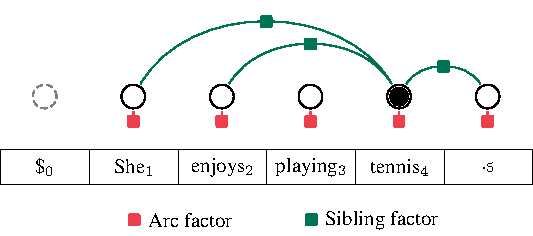
\includegraphics[scale=1]{figures/dep-factors.pdf}
    \caption{依存句法模型的因子图}
    \label{fig:dep-factors}
  \end{subfigure}
  \begin{subfigure}[b]{0.8\textwidth}
    \centering
    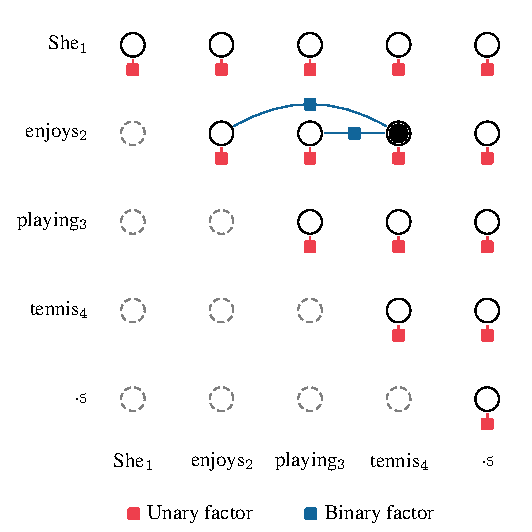
\includegraphics[scale=1]{figures/con-factors.pdf}
    \caption{成分句法模型的因子图}
    \label{fig:con-factors}
  \end{subfigure}
  \caption{一个例句和其依存/成分句法模型对应的因子图,我们在例句上方标出了对应的正确无标签依存句法树和成分句法树,其中成分句法树进行了左二叉化.
    灰色虚线圆圈代表被屏蔽的变量.
    图中标出了所有的一阶(红色)因子,为了简洁起见,对于二阶因子,依存句法图中我们只标出了涉及弧$3\rightarrow 4$的兄弟(绿色)因子,成分句法图中只标出了和组块$(3, 4)$连接的二阶(蓝色)因子.}
  \label{fig:vi-factors}
\end{figure}

在得到分值之后,我们的句法分析方法分为两阶段:1)构建无标签树;2)预测标签.
在第二阶段预测标签的时候,我们以贪婪的方式给依存树的每条弧(见章节~\ref{sub@sec:dep-crf-labeling})或者成分树的每个组块(见章节~\ref{sub@sec:con-crf-model-definition})打上标签.
而在第一阶段构建无标签树时,我们的目的是选择后验概率最大的句法树$\boldsymbol{y} = \arg\max_{\boldsymbol{y}^{\prime}} P(\boldsymbol{y}^{\prime}\mid \boldsymbol{x})$.
通常这样的推断的复杂度较高,以至于无法计算.
在句法分析领域我们可以应用复杂度为$O(n^3)$的Inside算法来进行精确计算,尽管在前面章节我们展示了可以通过批次化以及张量并行计算来降低复杂度,但是仍然十分影响计算效率.
因此在本节我们提出利用基于平均场理论的变分推断法(Mean Field Variational Inference, \textsc{Mfvi})来近似得到后验概率.
\textsc{Mfvi}假设句法树$\boldsymbol{y}$每个位置的变量相互独立,因此可以在线性时间内通过迭代的方法得到后验概率的近似值$Q(\boldsymbol{y})$.

关于\textsc{Mfvi}的通用更新公式以及相关推导见附录~\ref{appendix:mfvi-derivation}.
根据依存句法和成分句法任务目标的不同,我们在下面两小节详细阐述了通用公式针对具体任务的特化版本,以及相关的势函数(potential function)和因子图(factor graph)的设计.

\noindent\textbf{基于头选择的变分推断.}
目前广泛使用的一阶局部模型(对应于章节~\ref{cha:dep-crf}的\textsc{Loc}方法,这里我们称为\textsc{Loc}$_{dep}$)在训练的时候采用了头选择(head selection)训练目标,要求句子中除了根结点之外的每个词有且仅有一个头.
和\citep{wang-tu-2020-second}一样,我们选择在依存句法对应变分推断方法中引入头选择约束,相应的因子图见图~\ref{fig:dep-factors}..
对于每个位置$j$,我们定义变量取值为$y_j\in \{0,1,\cdots,i\neq j,\cdots,n\}$,代表词$w_j$的可能的头索引.

具体地,对于每个变量$y_j$,一阶的势函数定义为
\begin{equation}
  \label{eq:dep-1o-potential}
  \psi_j(y_j)=\exp(s(y_j\rightarrow j))
\end{equation}
$s(y_j\rightarrow j)$是弧$y_j\rightarrow j$对应的分值,由公式~\ref{eq:biaffine}计算得到.

对于两个变量$y_{j}$和$y_{k}$,我们使用和章节~\ref{cha:dep-crf}一致的二阶特征,对应的二阶势函数定义为
\begin{equation}
  \label{eq:2o-dep-potential}
  \psi_{j,k}(y_j,y_k)=\left\{
  \begin{array}{rcl}
    \exp \mathrm{s}(y_j\rightarrow \{k,j\}) &  & {y_j=y_k}   \\
    1                                       &  & {otherwise}
  \end{array}
  \right.
\end{equation}
$s(y_j\rightarrow \{k,j\})$是兄弟子树$y_j\rightarrow \{k,j\}$的分值,由公式~\ref{eq:triaffine}计算得到.
需要注意的是这里的兄弟$k$和二阶TreeCRF不一样,并不需要一定和$j$邻近.

\textsc{Mfvi}迭代式地更新近似分布$Q(\cdot)$,来最小化其与真实分布$P(\cdot)$的KL散度,依存句法模型的迭代更新公式如下\citep{wang-tu-2020-second}:
\begin{equation}
  \label{eq:mfvi-dep}
  Q_{j}^{(t)}(i)\propto \exp\left(s(i\rightarrow j) +\sum_{k\neq i,j} Q_{k}^{(t-1)}(i)\cdot s(i\rightarrow {k,j}) \right)
\end{equation}
后验概率$Q_j^{(0)}(i)$初始化为一阶势函数$\psi_j(i)$.
每次迭代时,我们都会将$Q_j^{(0)}(\cdot)$的值在所有可能的头取值上进行归一化.

\noindent\textbf{基于二分类的变分推断.}
我们的成分句法分析模型采用了\citep{gaddy-etal-2018-whats}的方法作为基线方法,称为\textsc{Loc}$_{con}$.
具体来说,模型对短语树所有可能的位置进行一个简单的二分类,预测该位置是否是一个区块.
\citep{dozat-manning-2018-simpler,wang-etal-2019-second}在语义依存分析中应用了这样的训练目标.
\citep{gormley-eisner-2015-structured,naradowsky-etal-2012-grammarless}在成分句法分析中应用了这种方法,并采用循环置信传播(Loopy Belief Propagation, LBP)来近似获得后验概率,并设计了若干种局部和全局因子,比如\textsc{Exactly1}、\textsc{Tree}等.
我们将其引入到了基于\textsc{Mfvi}的成分句法分析中,但是简单起见仅仅采用了一个一阶因子和一个二阶因子,对应的因子图见图~\ref{fig:con-factors}.
我们考虑将引入更多因子约束的近似算法留待作为未来工作.


具体地,每个位置$ij$的可能的变量取值$y_{ij}\in \{0,1\}$. 对于单个变量$y_{ij}$,一阶的势函数定义为
\begin{equation}
  \label{eq:con-1o-potential}
  \psi_{ij}(y_{ij})=\left\{
  \begin{array}{rcl}
    \exp\left(\mathrm{s}(i,j)\right) &  & {y_{ij}=1}  \\
    1                                &  & {otherwise}
  \end{array}
  \right.
\end{equation}
$s(i,j)$是区块$(i,j)$的分值,由公式~\ref{eq:con-biaffine}计算得到,这里我们要求$i<j$.

给定两个变量$y_{ij}$和$y_{lk}$,我们考虑使用和章节~\ref{cha:con-crf}一致的二阶兄弟特征,因此二阶的势函数定义为
\begin{equation}
  \label{eq:2o-con-potential}
  \psi_{ij,lk}(y_{ij},y_{lk})=\left\{
  \begin{array}{rcl}
    \exp\left(\mathrm{s}(i,k,j)\right) &  & {i=l}       \\
    1                                  &  & {otherwise}
  \end{array}
  \right.
\end{equation}
$s(i,k,j)$可以视为$(i,j)$和$(i,k)$都作为组块时,组成的子树的分值,由公式~\ref{eq:con-triaffine}计算得到,这里$k$的位置不受动态规划算法的约束,并不要求一定位于$(i,j)$之间,即有$i<j,k$.

成分句法模型的\textsc{Mfvi}迭代更新公式如下:
\begin{equation}
  \label{eq:mfvi-con}
  \begin{array}{l}
    Q_{ij}^{(t)}(0)\propto 1 \\
    Q_{ij}^{(t)}(1)\propto \exp\left(s(i,j) +\sum_{k\neq i,j} Q_{ik}^{(t-1)}(1)\cdot s(i,k,j) \right)
  \end{array}
\end{equation}
后验概率$Q_{ij}^{(0)}(y_{ij})$初始化为一阶势函数$\psi_{ij}(y_{ij})$.
每次迭代时,我们将$Q_{ij}^{(0)}(\cdot)$在取值$\{0,1\}$上进行归一化.


\subsection{训练}

我们的训练损失函数分为两部分,分别是无标签树的损失和对应标签的损失.
给定所有正确标签,我们的目标是最大化树上每个标签的概率,和前面的章节一致,我们采用了弧/区块级别的标准交叉熵损失函数.
给定输入句子$\boldsymbol{x}$和对应正确的无标签句法树$\boldsymbol{y}^{\ast}$,我们的目标是最大化句法树的概率$P(\boldsymbol{y}^{\ast}\mid\boldsymbol{x})$.
由于\textsc{Mfvi}将概率在每个变量上分解,得到近似概率$Q(\boldsymbol{y}^{\ast})$,因此训练目标等价于最大化每个变量的后验概率.

对于每个句子,依存句法分析相应无标签句法树的目标函数为
\begin{equation}
  \label{eq:dep-vi-arc-loss}
  L_{dep}^{arc}=-\sum_{j\neq 0}\log Q_j(\boldsymbol{y}^{\ast}_j)
\end{equation}

成分句法的无标签句法树的目标函数为
\begin{equation}
  \label{eq:con-vi-bracket-loss}
  L_{con}^{bracket}=-\sum_{i<j}\log Q_{ij}(\boldsymbol{y}^{\ast}_{ij})
\end{equation}
对于最终的目标函数,我们新引入了一个参数$\lambda$用于平衡无标签句法树以及标签的损失,相应的最终训练目标为
\begin{equation}
  \label{eq:con-vi-loss}
  L_{con}=\lambda L_{con}^{label}+(1-\lambda)L_{con}^{bracket}
\end{equation}

\subsection{解码}
在\textsc{Mfvi}模型中,解码时我们直接应用了MBR解码.
我们直接用\textsc{Mfvi}近似得到的后验概率作为解码算法的输入.
依存句法中,我们将由公式~\ref{eq:mfvi-dep}得到的概率$Q_i(\cdot)$作为输入,并利用了Eisner算法来解码,加速时采用了算法~\ref{alg:eisner-2o}的批次化技术.
成分句法中,我们将由公式~\ref{eq:mfvi-con}得到的概率$Q_{ij}(\cdot)$作为输入,并利用了和章节~\ref{cha:con-crf}一样的类CKY算法来解码,采用了算法~\ref{alg:inside}的批次化技术来加速.


\section{实验}\label{sec:vi-exp}

\noindent\textbf{数据.}
为了方面和章节~\ref{cha:dep-crf}提出的精确推断的高阶模型进行比较,我们主要在英文的PTB和中文的CNLL09上进行了依存句法的实验.
同样的,我们在英文的PTB,中文的CTB51以及CTB7进行了成分句法分析实验.
实验数据的详细设置在章节~\ref{cha:dep-crf}和章节~\ref{cha:con-crf}有详细的设置,这里简洁起见不再重复.

\noindent\textbf{评价.}
在依存句法分析上,我们主要采用了有标签和无标签附着分值(UAS/LAS)作为评价指标,英文PTB的标点被忽略.
在成分句法分析上,我们采用了惯用的区块级别的准确率、召回率和$\mathrm{F}_1$值(P/R/$\mathrm{F}_1$)的指标,由标准工具\texttt{EVALB}来得到.
成分句法树在训练和评价时采用的预处理和后处理行为我们保持和章节~\ref{cha:con-crf}一致.

\noindent\textbf{参数设置.}
我们保持两种句法分析模型的编码器和训练方法与前面的章节基本一致.
对于二阶模型,我们设置依存句法分析中使用的兄弟特征以及成分句法分析使用的二阶特征的MLP层输出维度为100.
我们设置变分推断的迭代次数统一为3次.
对于在成分句法分析中的用于平衡标签和无标签树的训练损失的参数$\lambda$,我们设置$\lambda$为0.1.

\begin{table}[tb!]
  \centering
  \caption{依存句法分析模型在PTB和CoNLL09的Test数据上不同推断算法的结果.}
  \begin{tabular}{lcccc}
    \toprule
                   & \multicolumn{2}{c}{PTB} & \multicolumn{2}{c}{CoNLL09}                                   \\
                   & UAS                     & LAS                         & UAS            & LAS            \\[2pt]
    \midrule
    \\[-15pt]
    \textsc{Loc}   & 96.08                   & 94.47                       & 89.15          & 85.98          \\
    \textsc{Crf}   & 96.02                   & 94.33                       & 89.28          & 86.18          \\
    \textsc{Mfvi}  & \textbf{96.11}          & \textbf{94.49}              & 89.35          & 86.25          \\
    \textsc{Crf2o} & \textbf{96.11}          & 94.46                       & \textbf{89.63} & \textbf{86.52} \\
    \multicolumn{5}{c}{+BERT}                                                                                \\[3pt]
    \textsc{Loc}   &                                                                                         \\
    \textsc{Crf}   &                                                                                         \\
    \textsc{Mfvi}  &                                                                                         \\
    \textsc{Crf2o} &                                                                                         \\
    \bottomrule
  \end{tabular}
  \label{table:vi-dep-test}
\end{table}




\subsection{结果}
表格~\ref{table:vi-dep-test}和表格~\ref{table:vi-con-test}分别给出了我们尝试的多种推断算法在依存句法和成分句法分析上的比较性实验结果.
和章节~\ref{cha:dep-crf}以及章节~\ref{cha:con-crf}一样,我们在所有模型中都使用了预训练词向量作为输入.
英文数据我们统一使用了100维的Glove词向量,中文数据则使用了word2vec在Giga数据上训练的100维词向.
我们还汇报了BERT的结果,对于英文数据,我们使用了24层1024维的\texttt{bert-large-cased}作为双向LSTM的输入,并在训练时固定参数.
中文数据我们则使用了12层768维的\texttt{bert-base-chinese}.

可以看到在依存句法的结果上(表格~\ref{table:vi-dep-test}),由于英文PTB的结果非常高,因此这四种推断方法的结果都十分接近,\textsc{MFVI}方法超越了\textsc{Loc},达到了最好的性能.
中文CoNLL09上,精确推断的\textsc{Crf2o}仍然是最好的,但是\textsc{MFVI}超越了\textsc{Crf}达到了86.25的LAS.
在两种语言上,\textsc{MFVI}都一致超越了没有全局结构约束的\textsc{Loc}方法.
这验证了在近似推断的\textsc{MFVI}方法上应用二阶结构约束的有效性.

在成分句法分析上(表格~\ref{table:vi-con-test}),中英文三个数据的结果中,无论是一阶\textsc{Crf}还是二阶\textsc{Crf2o},精确推断算法都仍然是表现最好的.
然而\textsc{Mfvi}都达到了和一阶\textsc{Crf}十分相近的性能.
并且,\textsc{Mfvi}一致超越了基于二分类学习的\textsc{Loc}模型,在PTB、CTB51和CTB7上分别提升了0.11、0.52和0.35.

当使用BERT之后,上述的几种推断算法在结果上没有显著差异.
依存句法上,PTB中\textsc{Mfvi}表现最好,LAS为95.37,达到或超越了当前的最佳性能\citep{zhou-zhao-2019-head,wang-tu-2020-second},CoNLL09上人仍然\textsc{Crf2o}最佳,但是\textsc{Mfvi}的差距十分微弱.
成分句法中在PTB和CTB51这两个数据上,\textsc{Mfvi}的表现都是最好的,分别达到95.71和92.56的$\mathrm{F}_1$值,高于当前最佳的模型\cite{kitaev-etal-2019-multilingual}.
在CTB7上表现最好的仍是\textsc{Crf2o},$\mathrm{F}_1$值为91.62,而\textsc{Mfvi}的差距不到0.1.
然而,基于\textsc{Mfvi}方法的近似推断在解析效率上有很大的优越性(见章节~\ref{sub@sec:vi-speed}的复杂度分析).

\begin{table}[tb!]
  \centering
  \caption{成分句法分析模型在英文PTB、中文CTB5.1和CTB7的Test数据上不同推断算法的结果.}
  \begin{tabular}{lccccccccc}
    \toprule
                   & \multicolumn{3}{c}{PTB} & \multicolumn{3}{c}{CTB51} & \multicolumn{3}{c}{CTB7}                                                                                                       \\
                   & $\mathrm{P}$            & $\mathrm{R}$              & $\mathrm{F}_1$           & $\mathrm{P}$   & $\mathrm{R}$   & $\mathrm{F}_1$ & $\mathrm{P}$   & $\mathrm{R}$   & $\mathrm{F}_1$ \\[2pt]
    \midrule
    \\[-15pt]
    \textsc{Loc}   & 94.16                   & 93.85                     & 94.01                    & 89.39          & 89.16          & 89.28          & 88.54          & 87.96          & 88.25          \\
    \textsc{Crf}   & 94.23                   & 94.02                     & 94.12                    & 89.71          & \textbf{89.89} & 89.80          & 88.84          & 88.36          & 88.60          \\
    \textsc{Mfvi}  & 94.11                   & 93.96                     & 94.04                    & 89.82          & 89.79          & \textbf{89.81} & 88.71          & 88.16          & 88.43          \\
    \textsc{Crf2o} & \textbf{94.29}          & \textbf{94.15}            & \textbf{94.22}           & \textbf{89.97} & 89.47          & 89.72          & \textbf{88.95} & \textbf{88.56} & \textbf{88.76} \\
    \multicolumn{10}{c}{+BERT}                                                                                                                                                                            \\[3pt]
    \textsc{Loc}   & 95.70                   & 95.43                     & 95.57                    & 92.47          & 92.09          & 92.28          & 91.90          & 91.24          & 91.57          \\
    \textsc{Crf}   & 95.85                   & 95.53                     & 95.69                    & 92.51          & 92.04          & 92.27          & 91.73          & \textbf{91.38} & 91.55          \\
    \textsc{Mfvi}  & 95.85                   & \textbf{95.57}            & \textbf{95.71}           & \textbf{92.78} & \textbf{92.35} & \textbf{92.56} & 91.89          & 91.31          & 91.60          \\
    \textsc{Crf2o} & \textbf{95.86}          & 95.47                     & 95.67                    & 92.75          & 92.18          & 92.47          & \textbf{91.93} & 91.31          & \textbf{91.62} \\
    \bottomrule
  \end{tabular}
  \label{table:vi-con-test}
\end{table}



% \subsection{分析}


\subsection{样例学习}

\begin{figure}[tb!]
  \centering
  \begin{subfigure}[b]{0.9\textwidth}
    \centering
    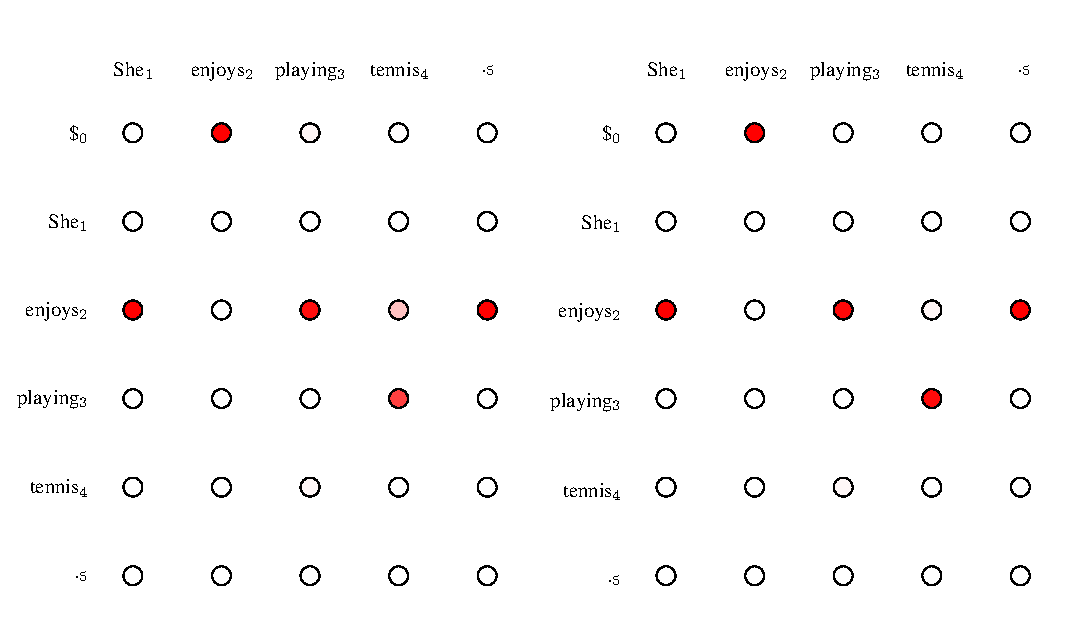
\includegraphics[scale=0.75]{figures/dep-probs.pdf}
    \caption{依存句法树每个位置对应的分值和后验概率}
    \label{fig:dep-probs}
  \end{subfigure}
  \begin{subfigure}[b]{0.9\textwidth}
    \centering
    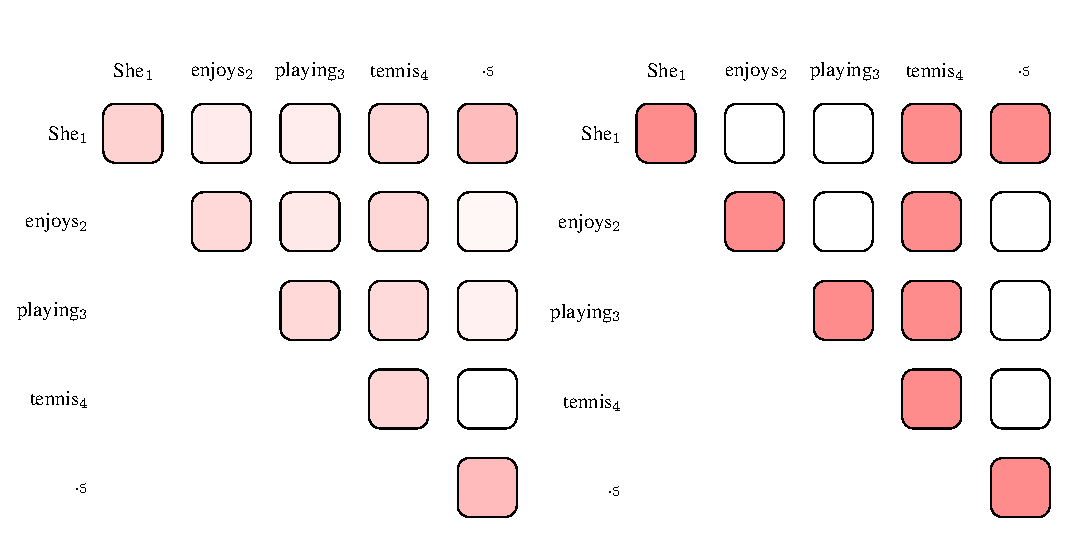
\includegraphics[scale=0.75]{figures/con-probs.pdf}
    \caption{成分句法树每个位置对应的分值和后验概率}
    \label{fig:con-probs}
  \end{subfigure}
  \caption{一个例句对应的依存句法模型和成分句法模型的输出. 左边的图是每个位置的分值(log potential),为了方便显示,我们首先对分值进行了归一化.
    右边的图是变分推断得到的后验概率. 灰色虚线圆圈代表被屏蔽的不合法位置.}

  \label{fig:vi-probs}
\end{figure}

图~\ref{fig:vi-probs}给出了一个例句分别在依存和成分句法模型上的分值(log potentials)与经过\textsc{Mfvi}迭代近似得到的后验概率的热力图对比.
图中颜色的深浅反应了分值/概率的大小.

左边的图反应的是模型直接输出的分值之间的对比,这对应于一阶模型的输出.
可以看到模型的输出的分值数值相对来说都比较均匀.
由于依存句法模型基于的是头选择的训练目标,可以看到图中的每一列都有一个极值存在,比如词$She_i$对应的列中,颜色最深(分值最高)的位置为词$enjoys_2$,这对应了句法树中的弧$enjoys_2\rightarrow She_1$.
成分句法的热力图中,由于采用了二分类的目标,因此颜色较深的位置表示更可能成为一个区块.
然而由于没有类似于依存句法的头约束,直接通过对每个位置$\arg\max$得到的所有区块可能无法组成一棵合法的句法树,因此我们仍需要CKY算法来获得全局最优的合法句法树.

当我们利用\textsc{Mfvi}算法,得到的近似后验概率的热力图如右边图所示.
可以看到,在进一步考虑了二阶特征的分值并聚合到每个变量位置之后,后验概率的置信度远远高于分值.
对于依存句法而言,每个词都有一个最可能的头,并且概率几乎为1,对应于热力图中每列仅有一个红色结点.
对于成分句法而言,如果对图中每个位置的后验概率取$\arg\max$得到可能的区块,每个区块的概率同样近似为1,并且对于图中的例句而言,这种贪婪解码得到的句法树可以直接组成一棵合法的短语结构树,例如,红色结点$(She_1,tennis_4)$和$(playing_3,tennis_4)$对应了例句正确的无标签树左二叉化之后的两个区块.
这显示了\textsc{Mfvi}在引入二阶结构打分之后,对于模型结构预测更强大的约束作用.


\subsection{速度和时间复杂度比较}
\label{sub@sec:vi-speed}
\begin{table}[tb!]
  \centering
  \caption{依存句法和成分句法使用不同推断算法的时间复杂度,以及相应的在PTB的Test数据上的解析时间的比较.
    依存句法统一使用了Eisner算法解码,成分句法统一使用了CKY算法解码}
  \begin{tabular}{llcccr}
    \toprule
     & \multirow{2}{*}{Inference} & \multicolumn{2}{c}{Complexity} & \multirow{2}{*}{Decoding Alg.} & \multirow{2}{*}{Sents/sec}                 \\
     &                            & CPU                            & GPU                            &                            &               \\[2pt]
    \midrule
    \multirow{3}{*}{Dependency}
    % & \textsc{Loc}               & $O(n)$                         & $O(1)$                         & Eisner                     & 990           \\
     & \textsc{Crf}               & $O(n^3)$                       & $O(n^2)$                       & Eisner                     & 653           \\
     & \textsc{Crf2o}             & $O(n^3)$                       & $O(n^2)$                       & Eisner                     & 431           \\
     & \textsc{Mfvi}              & $O(n^3)$                       & $O(n)$                         & Eisner                     & \textbf{1126} \\
    \midrule
    \multirow{3}{*}{Constituency}
    % & \textsc{Loc}               & $O(n)$                         & $O(1)$                         & CKY                        & 990           \\
     & \textsc{Crf}               & $O(n^3)$                       & $O(n^2)$                       & CKY                        & 743           \\
     & \textsc{Crf2o}             & $O(n^3)$                       & $O(n^2)$                       & CKY                        & 598           \\
     & \textsc{Mfvi}              & $O(n^3)$                       & $O(n)$                         & CKY                        & \textbf{905}  \\

    \bottomrule
  \end{tabular}
  \label{table:vi-speed}
\end{table}
表~\ref{table:vi-speed}给出了\textsc{Mfvi}和前面章节提及的精确推断模型的速度和复杂度的比较.
为了统一比较,所有的设置下都应用了MBR解码,并且每个任务都用了相同的解码算法.
可以看到,无论是依存句法还是成分句法模型,他们相应的\textsc{Mfvi}在CPU上每一次迭代都需要$O(n^3)$的复杂度,这和精确推断的2阶Inside算法的复杂度相当.
而当利用GPU进行并行计算时,\textsc{Mfvi}每个位置的变量仅需要一次遍历来收集其他位置的信息\footnote{尽管现代的CUDA技术可以通过二叉树等数据结构让并行化的归约操作,例如$\mathrm{sum}$、$\mathrm{min}$和$\mathrm{max}$等,缩减到$O(\log n)$复杂度的时间\citep{wang-etal-2020-ain},但是这里我们统一假设归约操作的复杂度为$O(n)$.},因此GPU上的算法复杂度为$O(n)$,大大快于精确推断所需要的$O(n^2)$复杂度.

从表中可以看到,利用\textsc{Mfvi}的依存句法在PTB的Test数据的解析速度为1126句/秒,是精确推断的二阶\textsc{Crf2o}(431)的近三倍快,同样也大大快于一阶\textsc{Crf}的653句/秒.
成分句法的\textsc{Mfvi}模型的解析速度大约为905句/秒,同样显著快于一阶\textsc{Crf}的743句/秒和二阶\textsc{Crf2o}的598句/秒.

\section{本章小结}

在本章我们将包含二阶特征的\textsc{Mfvi}方法方法引入到了依存句法和成分句法分析中.
根据两种句法分析的特点,在依存句法分析上,我们参考\citep{wang-tu-2020-second}实现了一个包含头选择约束的\textsc{Mfvi}方法,在成分句法分析上,我们引入了一个基于二分类学习目标的\textsc{Mfvi}方法.
在这两个任务的中英文个五个数据集上的结果表明,\textsc{Mfvi}方法均超越了基于局部学习的\textsc{Loc}方法,并达到和精确推断的二阶\textsc{Crf2o}方法可比较的性能.
此外\textsc{Mfvi}方法相比于精确推断的解析速度大大加快.
在加入BERT之后,基于\textsc{Mfvi}方法的近似推断模型在所有的数据集上都达到或者接近了当前最佳的模型.